As was mentioned above, surface extraction is an intermediate step after Topology Optimization and NURBS representation in order to facilitate the conversion. In terms of implementing the surface extraction, we used VTK \cite{VTKToolbox}.

%\subsection{VTK Toolbox}


%The VTK toolbox was used in order to implement the algorithms on our optimized data. It is a heavily object
%oriented toolbox. Our first approach was to use the built in Marching Cubes algorithm,
%nevertheless it did not work with our unstructured grid data. It just works for ImageData and
%PolyData . For structured and unstructured grids the tool to render the isosurface is the \textit{Contour Filter} tool. Unfortunately the documentation does not present which algorithm the tool uses. It
%can be inferred that it is an extended Marching cubes algorithm.

The VTK Toolbox is an open-source tool, providing algorithms for "3D computer graphics, image processing, and visualization" \cite{VTKToolbox}. Among the variety of tools, VTK offers algorithms that allow us to obtain a surface representation from voxel data. Among these algorithms, we could find Marching Cubes, Dual Contouring and also a Decimation tool, the last of which can useful for reducing the data size further for the NURBS-representation step.


%\subsection{Implementation}
The \textit{Marching Cubes} implementation in VTK is however not applicable to our the Unstructured Grid data that we obtain from ToPy, since it only works with ImageData and PolyData, the main data types in VTK. For structured and unstructured grids the tool to render the isosurface is the \textit{Contour Filter} tool. Unfortunately, the documentation does not present which algorithm the tool uses. It can be inferred that it is an extended \textit{Marching Cubes} algorithm. %how?
Although an implementation with \textit{Contour Filtering} worked, the visualization of the data was still not possible
making an intermediate step needed. Here, we used the \textit{Implicit Modelling} tool, a filter that
computes the distance from the input geometry to the points of an output structured point set.
This distance function can then be "contoured" to generate new, offset surfaces from the original
geometry. Although this approach allowed the visualisation, some crucial information was lost, as for example holes were not represented in the final model. The result can be shown in \autoref{fig:contouring}.


\begin{figure}
\centering
   \scalebox{0.4}{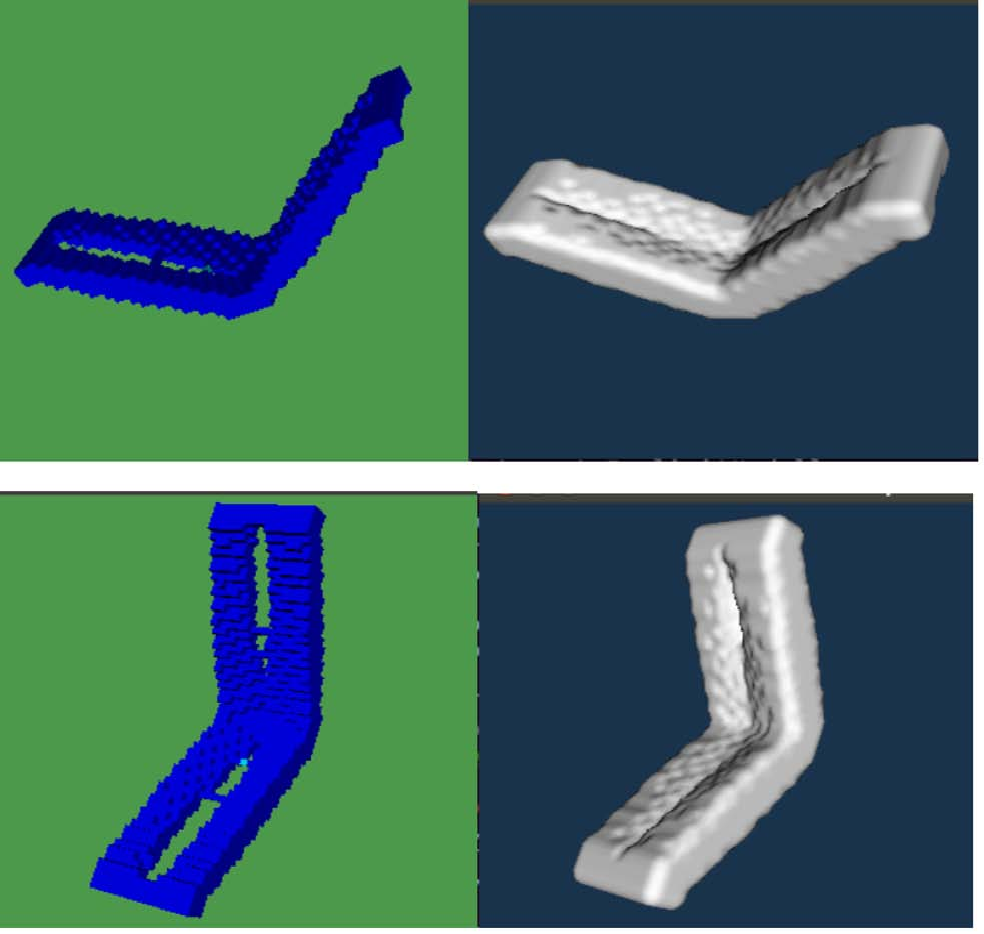
\includegraphics{Pictures/contouring.pdf}}\\
   \caption{Contour Filtering tool after Implicit Modelling. The original geometry (left) is an optimized geometry output from \emph{ToPy} (see \autoref{sec:ToPy}. Note that some essential features of the geometry after the process (right) are lost, such as the holes through the structure.}
   \label{fig:contouring}
\end{figure}

% I don't understand this sentence - I'll leave it out for now.

%A further idea to solve this problem is to first convert the volume data into point data
%and only then present it to the \textit{Contour Filtering} tool .

In order to reduce computational costs of the following \emph{NURBS fitting} process (see \autoref{sec:NURBS}) we also need to create a coarser mesh of polygons from the fine one. The number of triangles that represent the
isosurface can here be reduced with the VTK \emph{Decimation} tool mentioned above. A smoothing step is however necessary in-between
to get the new connections right. As can be seen in \autoref{fig:Decimation}, a 50 \% reduction of the
triangles barely provides a noticeable difference, and even with a 90 \% reduction it is difficult to see a difference. Triangle meshes can be easily coarsened since there are many open source algorithms that reduce the number of triangles. %reference

\begin{figure}
\centering
   \scalebox{0.4}{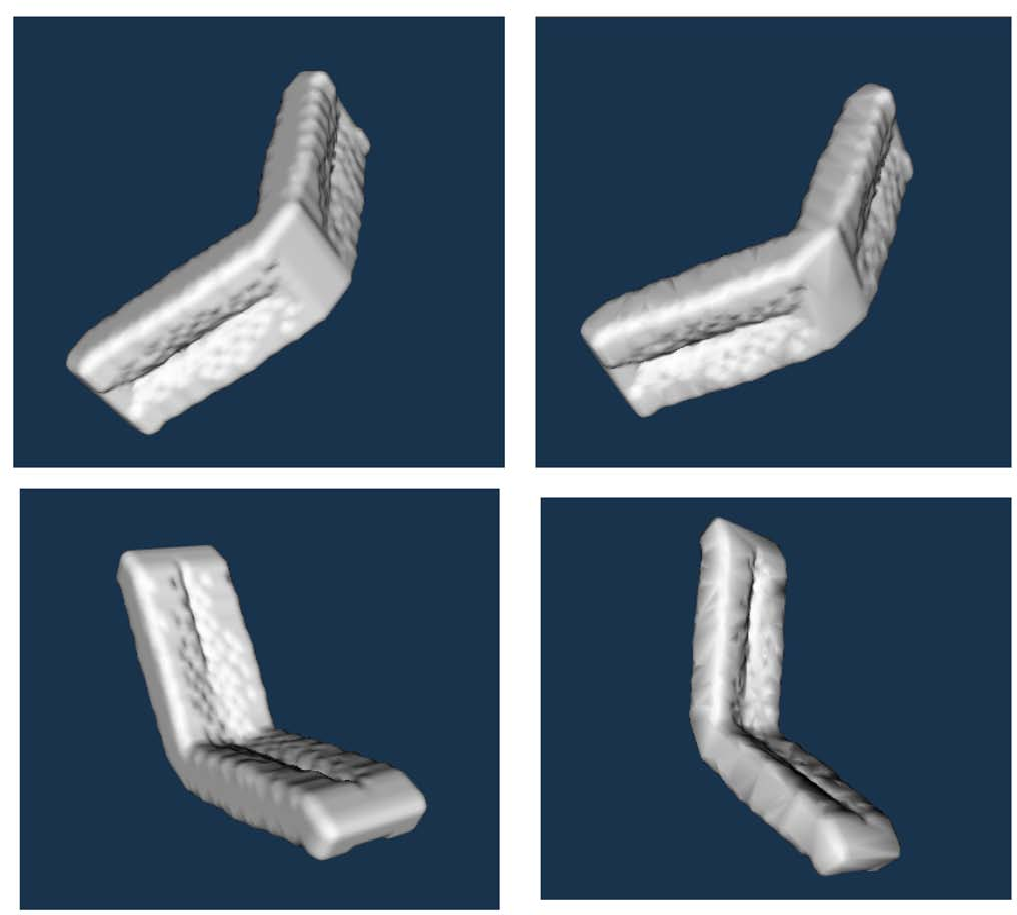
\includegraphics{Pictures/Decimation.pdf}}\\
   \caption{Decimation of triangles. \emph{Top:} 50\% reduction of triangle number from the object in \autoref{fig:contouring}. \emph{Lower:} 90\% reduction. The difference is barely noticable in both cases.}
   \label{fig:Decimation}
\end{figure}
